\documentclass[Afour,sageh.bst]{sagej}

\usepackage{moreverb,url,natbib, multirow, tabularx}
\usepackage[colorlinks,bookmarksopen,bookmarksnumbered,citecolor=red,urlcolor=red]{hyperref}


\usepackage{natbib}

\usepackage{bm}
     \def\Var{{\rm Var}\,}
     \def\Cov{{\rm Cov}\,}
     \def\mean{{\rm mean}\,}
     \def\E{{\rm E}\,}
  	 \def\Corr{{\rm Corr}\,}
\newcommand{\vect}[1]{\boldsymbol{#1}}


\usepackage{hyperref}
\usepackage{rotating}
\usepackage{booktabs}
\usepackage{makecell}


\begin{document}

\title{Modeling the impacts of park access on health outcomes: a utility-based
accessibility approach}

\runninghead{XXXX \emph{et al}.}

\author{XXXX \affilnum{1}, XXXX \affilnum{2}, XXXX\affilnum{3}, XXXX\affilnum{3}}

\affiliation{
\affilnum{1}{XXXX}\\
\affilnum{2}{XXXX}\\
\affilnum{3}{XXXX}}

\corrauth{XXXX}

\email{\href{XXXX}{\nolinkurl{XXXX}}}

\begin{abstract}
Recent research has underscored the potential for public green spaces to
influence individual and societal health outcomes, but empirical
measurements of such influences have yielded mixed results to date, with
particular disagreement surrounding how access to parks ought to be
defined while controlling for alternate explanations. In this paper we
apply a comprehensive measure of park accessibility drawn from random
utility choice theory, which avoids arbitrary assertions of proximity
while incorporating potentially numerous amenities and attributes of
both the parks and the population. We apply this utility-based
accessibility measure to correlate Census tract-level obesity and
physical activity rate estimates from the Centers for Disease Control
and Prevention's 500 Cities project with tract-level American Community
Survey socioeconomic data in New York City, paired with geographic open
space data from New York City. Controlling for the socioeconomic
variables and spatially correlated error terms, we show a positive and
significant relationship between park access and physical activity
rates. The data also suggest a negative relationship between park access
and obesity rates, beyond what is expected through physical activity and
socioeconomics. In doing so, this research contributes a more
comprehensive modeling approach for measuring the impact of park access
on health, and may improve our understanding of the role parks and
access to them can serve in furthering public health objectives.
\end{abstract}

\keywords{Accessibility; Green Space; Public Health}

\maketitle

\clearpage
\newpage
\hypertarget{introduction}{%
\section{Introduction}\label{introduction}}

The United States and other developed nations face an epidemic of
obesity and chronic diseases, including cardiovascular diseases, chronic
respiratory diseases, diabetes, stroke, joint and bone diseases, and
cancer. These diseases can severely limit the lifespan of affected
individuals \citep{WHO2014}, with substantial financial costs for
treatment borne both privately and socially \citep{Finkelstein2009}.
Though a moderate amount of regular physical activity has been
established as an effective strategy for reducing and managing obesity
and many of the aforementioned chronic diseases
\citep{CDC2009, Durstine2013}, a large portion of U.S. adults do not
participate in sufficient physical activity \citep{Wolf2008}.

Historically, most large-scale health promotion efforts focused on
individual-level interventions intended to educate people about healthy
lifestyles and behaviors, touching on topics including diet and
exercise. Over the last several years a new \emph{social} model of
health has evolved, described by \citet{Duhl1999} ``as an outcome of the
effects of socioeconomic status, culture, environmental conditions,
housing, employment and community
influences''\citeyearpar[p.7]{Duhl1999}. In this new paradigm, resources
provided via civil infrastructure --- in particular parks and other
public green spaces --- play a crucial role in promoting and sustaining
public health \citep{Bedimo-Rung2005, Wells2007, Coutts2008}. After all,
it does little to educate individuals on the importance of exercise if
their community is built in such a way that such exercise is expensive,
unenjoyable, or unsafe.

In spite of the potential for green spaces to influence public health
outcomes and numerous studies attempting to empirically estimate the
strength of these outcomes, evidence to date has been mixed. A major
challenge researchers have faced is a proliferation of techniques for
measuring access to green spaces, of which many are plausible but lack
robust theoretical bases. In this paper, we apply a holistic and
flexible measurement for park accessibility based in activity location
choice theory. This utility-based accessibility measure compares the
continuous distance to all parks in the region, weighted against the
sizes of each park and its other assorted amenities.

We apply this measurement to study the link between park accessibility
and attractiveness and census tract-level aggregate physical activity
participation and obesity rates in New York City, controlling for
spatially correlated unobserved effects, spatial spillovers of
covariates, and tract-level socioeconomic characteristics. We also
demonstrate how the utility-based accessibility metric can potentially
be expanded to account for other measures of a park's attractiveness
including its observed social media activity and the presence of various
park amenities. The paper concludes with a discussion of opportunities
for future research.

\hypertarget{literature-review}{%
\section{Literature Review}\label{literature-review}}

\label{sec:litreview}

The large majority of extant research on the topic of park access and
public health outcomes has been focused on comparing metropolitan
regions against each other. For example, \citet{West2012} used park data
from the Trust for Public Land's 2010 ``City Park Facts'' and public
health data from the Behavioral Risk Factor Surveillance System (BRFSS)
to examine the relationship between the density of park land and
physical activity and obesity rates for 67 metropolitan statistical
areas in the U.S. The findings in this case conformed to expectation;
that is, the study found a significant positive association between park
density and physical activity and a significant negative association
between park density and obesity. \citet{Larson2016} similarly used
self-reported scores on the Gallup-Healthways Wellbeing Index to
evaluate the relationship between physical health and park quantity,
quality, and accessibility in 44 U.S. cities. While the authors found
positive associations between wellbeing and park quality and
accessibility, these relationships were not statistically significant.
Conversely, \citet{Richardson2012} examined the relationship between
total urban greenspace and mortality rates for selected maladies; though
the authors did not find a statistically significant relationship
between the quantity of urban greenspace and mortality caused by lung
cancer, diabetes, heart disease or car accidents, they did find that
all-cause mortality was --- oddly --- \emph{higher} in greener cities.
Finally, in a meta-analysis of 20 peer reviewed journal articles
exploring the relationship between parks and objectively measured
physical activity, \citet{Bancroft2015} found that five studies reported
a significant positive association between the two, six studies produced
mixed results, and nine studies found no association at all.

Metropolitan-level analyses such as those described above do not capture
the within-city variation in accessibility to parks that exist in many
cities. Some cities with large amounts of total greenspace may
nevertheless unequally distribute this space throughout the city,
leading to areas with poor access. Conversely, a city with a smaller
overall proportion of greenspace may give all of its citizens better
access to sufficient greenspace to meet their needs or desires for
physical activity. Considering access at the neighborhood level within a
single city may also eliminate some regional or cultural fixed effects
affecting metropolitan-level analyses.

\hypertarget{park-accessibility-measures}{%
\subsection{Park Accessibility
Measures}\label{park-accessibility-measures}}

Loosely defined, the \emph{accessibility} of an arbitrary place
describes the ease with which people can accomplish activities there.
Accessibility is an abstract concept with tempting quantifiability
\citep{Handy1997}, perhaps explaining the proliferation of calculation
mechanisms. \citet{Dong2006} present a helpful mathematical heirarchy of
common mechanisms, which we follow here. Consider a person residing at
point \(i\) in a city with parks \(j \in 1 \ldots J\). An analyst might
consider point \(i\) as ``having access'' to a park if the distance to
the park \(d_{ij}\) is within an ``isochrone,'' or a geometric buffer
defined by some threshold \(D\),

\begin{equation}\label{eq:isochrone}
A_i = \begin{cases} 
      1 & d_{ij}\leq D\\
      0 & d_{ij} > D
   \end{cases}
\end{equation}

Variations of this isochrone-based framework are easily derived and
relatively common. ParkScore \citep{parkscore2019} is a sophisticated
application of this approach where \(D\) is a carefully calculated
10-minute network-bound walk, paired with a demographic analysis of
areas within and outside of this threshold. In other applications \(D\)
might be more variably defined, such as the presence or percent of green
space within a political or statistical boundary
\citep{Mitchell2008, Stark2014} or within a specific distance threshold
\citep{Kaczynski2014}. It is also possible to attenuate an isochrone
with various factors; for instance, \citet{Dias2019} considered road
safety perception as an extenuating factor in the effective distance to
a park.

In spite of the flexibility of adapted isochrone techniques, the
arbritrary definitions necessarily imposed by researchers in its
application can inhibit holistic analysis \citep{Logan2017}. A somewhat
more complete approach is the so-called ``gravity'' accessibility
statistic. In this case the accessibility of point \(i\) is the
denominator of the gravity formulation of a trip distribution model,
\begin{equation}\label{eq:gravity}
A_i = \sum_{j = 1}^J S_j f(d_{ij})
\end{equation} where \(S_j\) is the ``size'' of each park literally
(i.e.~acres) or abstractly (i.e. trip attractions) and \(f(d_{ij})\) is
a monotonically decreasing cost function, usually a negative
exponential. \citet{Dong2006} note that the isochrone framework is a
special case of the gravity model where \(f(d_{ij})\) is a binary
function and \(S_j = 1\). \citet{Giles-Corti2005} compare various
gravity-based accessibility scores with an isochrone specification and
show that the former are more predictive of walking behavior; that is,
the attributes of a park influence walking more than merely the distance
to it. \citet{Zhang2011} develop a population-weighted, gravity-based
accessibility to parks metric with a national scope, though they do not
examine its correlation with health outcomes.

A third accessibility mechanism is a utility-based specification, termed
as such for being derived from random utility choice theory. Consider
that an individual living at point \(i\) is choosing a park for a
recreation activity. If we apply the multinomial logit model
\citep{McFadden1974}, the expected consumer surplus enjoyed by this
individual can be shown to be \begin{equation}\label{eq:utility}
A_i = \ln\left({\sum_{j = 1}^J\exp(V_{ij})}\right) + C
\end{equation} where parks are differentiated from each other by their
relative measurable \emph{utilities}, \(V_{ij}\). \(C\) is an unknown
constant, but the difference in consumer surplus between two points
\(i\) and \(k\) can be quantitatively compared as \(A_i - A_k\)
\citep{Bruce1977}. In principle, \(V\) may include any measurable
attributes of either the choice maker or the park, and is typically
represented as a linear-in-parameters function of destination attributes
\(X_j\) and the travel cost \(d_{ij}\),
\begin{equation}\label{eq:utilityV}
V_{ij} = X_j\beta + \beta_d * d_{ij}
\end{equation} The coefficients \(\vect{\beta}\) are frequently
estimated from household surveys, though in the absence of a survey we
may assert reasonable values.

Note that the gravity formulation is itself a special case of the
utility-based specification where
\(\exp(X_j\beta + \beta_d d_{ij}) = X_j f(d_{ij})\) \citep{Daly1982}.
The distinction between gravity and utility-based specification is
meaningful, however. Primarily, it becomes possible to construct
accessibility statistics based on revealed behavioral preferences rather
than calibrated or asserted values \citep{Handy1997}.
\citet{Kaczynski2016} present what is effectively a utility-based
accessibility score they call ``ParkIndex'', with the explicit
motivation of developing a uniformly applicable park accessibility
statistic, though they limit this statistic as a way to add
heterogeneity within an isochrone analysis.

Both gravity and utility-based specifications hold several advantages
relative to isochrone-based accessibility metrics more commonly found in
the literature. First, all individuals are defined as having some access
to all parks, rather than an arbitrary cutoff asserted by the
researcher. This allows for the fact that some people are more or less
sensitive to distances, and that distance is a continuous, non-binary
phenomenon. It defies reason to assume a person living 11 minutes via
walking from a park always has meaningfully different accessibility than
someone living 9 minutes away. Second, the random utility formulation
allows the researcher to include -- in principle -- any attribute of the
park as part of its utility specification. This suggests that not all
parks are equal, and that a large park with many amenities such as
Central Park in Manhattan may provide health and activity benefits over
a much larger area than a smaller community square.

In spite of its flexibility and basis in choice theory, utility-based
accessibility measures have not received much application in the
accessibility literature compared with distance-based or even
gravity-based measures. \citet{Vale2016} present a descriptive
classification of active accessibility techniques, and explicitly
dismiss utility-based metrics for incorporating randomness. The
accessibility formula presented in Equation \ref{eq:utility} is the
expectation of a random utility process, and is not in and of itself
random any more than the gravity model is random. Utility-based
accessibility metrics are commonly used, however, in alternatives
analyses of transit infrastructure improvements \citep{DeJong2007}. A
reason for this is likely that a regional travel demand model is
available to the analysts, thus making calibrated and multimodal logsums
readily available \citep{Geurs2010}.

\hypertarget{empirical-application}{%
\section{Empirical Application}\label{empirical-application}}

In this section, we develop a model with data for New York City, where
we compute a set of utility-based accessibility to parks scores for each
tract and model the relationship between this measure and physical
activity rates, controlling for spatial effects and socioeconomic
factors. We subsequently model the effect of the accessibility metric on
obesity rates, accounting for physical activity and the other controls.

\hypertarget{data}{%
\subsection{Data}\label{data}}

This study uses data available to the public from a variety of federal
and state data agencies\footnote{The datasets, as well as the analysis
  code, are available on GitHub at
  \url{https://github.com/gregmacfarlane/parks_access}.}. The Centers
for Disease Control and Prevention makes small-area estimates on key
health indicators available through its 500 Cities data program
\citep{CDC5002016}. The indicators are multilevel aggregations and
imputations of BRFSS responses \citep{Wang2018, Wang2017}, and have been
recently used to study the tract-level link between gentrification and
urban health \citep{Gibbons2018}. We use two indicators as our dependent
variables in this study: the share of adults in a Census tract who are
obese, and the share of adults who participate in no leisure-time
physical activity. To improve clarity in our interpretation, we use the
complement of the second variable --- the share of tract adults who
participate in \emph{some} physical activity --- even if the amount may
not be sufficient to affect overall health. Both indicators are obtained
for the year 2016.

To the health data, we join socioeconomic data collected through the
Census Bureau API via the \texttt{tidycensus} package for R
\citep{Walker2019}. The primary dataset is a geographic polygons layer
of Census tracts in the five boroughs of New York City. We append to
each Census tract relevant socioeconomic data for each tract from the
American Community Survey 2013-2017 5-year estimates. For a small
handful of tracts in our sample, Census supressed the median income
estimate; these appear to be primarily wealthy tracts and in almost all
cases the CDC estimates of obesity and physical activity are missing as
well. After removing these tracts from the estimation dataset, we have
2,102 complete cases. Table \ref{tab:tractsdata} presents key
descriptive statistics for these data.

In a destination choice framework, the tracts represent the ``origins''
and the ``destinations'' are parks and green spaces in New York City. We
retrieved a polygons layer of public parks and greenspaces within New
York City's municipal boundaries and checked it for accuracy and
relevance \citep{nycparks}. Upon inspection, we removed several
facilities that do not qualify as publicly accessible green space, such
as Yankee Stadium, Citi Field, and their surrounding parking lots. We
also removed parks of less than half an acre in size, as these appear to
be predominantly planted medians rather than legitimate public green
space. We consolidated individual geographic polygons comprising a
single facility --- as is the case in Flushing Meadows --- and
eliminated sub-facilities such as tennis courts or baseball fields
included within larger park facilities. Instead of these distinct
sub-facilities, we created variables for each containing park indicating
the presence of sports courts, playgrounds, and trails.

To this dataset of parks and regularized green spaces, we add a polygons
layer of cemeteries in New York that are open to the public. Cemeteries
are important green spaces that can be used for many types of physical
activity. These operations leave us with 1,277 distinct green spaces;
for simplicity we will refer to both parks and cemeteries as ``parks''
going forward. For each park, we calculate the size of the park in
acres. Finally, using a Twitter application programming interface (API)
implemented with the Python package Tweepy, we also collected and stored
tweets containing geotags of precise geographic coordinates located
within the boundaries of the parks; from this information, we were able
to segregate tweets that were generated within a park in September 2014.
This geolocated twitter activity could provide an additional point of
information on the degree to which individual parks are actually used
\citep{Wang2016}.

\begin{table*}

\caption{\label{tab:tractsdata}Descriptive Statistics of Tract and Park Variables}
\centering
\resizebox{\linewidth}{!}{
\begin{tabular}[t]{l>{\raggedright\arraybackslash}p{2in}rlrl}
\toprule
  & Description & Minimum & Median (IQR) & Maximum & Source\\
\midrule
\addlinespace[0.3em]
\multicolumn{6}{l}{\textbf{Tract Variables, N = 2102}}\\
\hspace{1em}Obesity & Share of adults over 18 who are obese & 10.20 & \makecell{24.90\\ (19.83, 30.80)} & 45.40 & CDC 500 Cities\\
\hspace{1em}Physical Activity & Share of adults over 18 who engage in some leisure-time physical activity & 45.90 & \makecell{72.10\\ (66.60, 76.77)} & 90.70 & CDC 500 Cities\\
\hspace{1em}Income & Median tract income & 9053.00 & \makecell{59,592.50\\ (41,928.25, 79,092.75)} & 250001.00 & ACS\\
\hspace{1em}Density & Households per square kilometer & 9.20 & \makecell{5,848.46\\ (3,173.62, 9,674.36)} & 43621.52 & ACS\\
\hspace{1em}Fulltime & Share of adults over 18 with full-time work & 8.80 & \makecell{49.48\\ (44.45, 55.29)} & 100.00 & ACS\\
\hspace{1em}College & Share of adults over 24 with a college degree & 0.61 & \makecell{16.30\\ (12.37, 20.11)} & 44.94 & ACS\\
\hspace{1em}Single & Share of adults over 18 living alone or in a non-partnership household & 16.38 & \makecell{59.39\\ (50.30, 68.65)} & 100.00 & ACS\\
\hspace{1em}Youth & Share of population under 18 & 0.00 & \makecell{20.54\\ (16.79, 24.92)} & 64.07 & ACS\\
\hspace{1em}Young adults & Share of population between 18 and 34 & 0.00 & \makecell{25.73\\ (21.66, 29.98)} & 86.75 & ACS\\
\hspace{1em}Seniors & Share of population who are 65 and over & 0.00 & \makecell{12.83\\ (9.47, 16.88)} & 89.88 & ACS\\
\hspace{1em}Black & Share of population who is black & 0.00 & \makecell{10.03\\ (2.13, 44.62)} & 220.65 & ACS\\
\hspace{1em}Asian & Share of population who is Asian & 0.00 & \makecell{7.66\\ (2.40, 20.78)} & 88.07 & ACS\\
\hspace{1em}Hispanic & Share of population who is Hispanic & 0.00 & \makecell{19.07\\ (9.39, 41.07)} & 96.27 & ACS\\
\hspace{1em}Other & Share of population who belong to other minority groups & 0.00 & \makecell{0.00\\ (0.00, 0.53)} & 19.47 & ACS\\
\addlinespace[0.3em]
\multicolumn{6}{l}{\textbf{Park Variables, N = 1277}}\\
\hspace{1em}Size & Park size in acres & 0.50 & \makecell{1.66\\ (0.95, 5.62)} & 1961.00 & NYC\\
\hspace{1em}Courts & Presence of sport courts / ball fields & 0.00 & \makecell{0.00\\ (0.00, 0.00)} & 1.00 & NYC\\
\hspace{1em}Playgrounds & Presence of playgrounds & 0.00 & \makecell{0.00\\ (0.00, 1.00)} & 1.00 & NYC\\
\hspace{1em}Trails & Presence of trails & 0.00 & \makecell{0.00\\ (0.00, 0.00)} & 1.00 & NYC\\
\hspace{1em}Tweets & Tweets emanating from park in September 2014 & 0.00 & \makecell{0.00\\ (0.00, 2.00)} & 1593.00 & Twitter API\\
\bottomrule
\end{tabular}}
\end{table*}

\hypertarget{accessibility}{%
\subsection{Accessibility}\label{accessibility}}

\label{subsec:accessibility}

We calculate a set of utility-based accessibility statistics for each
tract in New York City. The most basic utility specification includes
only the park size in acres and the distance from the
population-weighted tract centroid to the boundary of the park in miles,
\begin{equation}\label{eq:u_access}
V_{ij} = \lambda_s * \log(size_j) + \lambda_d * \log(distance_{ij})
\end{equation} The logarithmic transform allows for diminishing marginal
utility of distance and park size: A 1-mile increase to a trip matters
more for a 1-mile trip than a 10-mile trip. \citet{Macfarlane2019}
estimated destination choice parameters for park trips in Alameda County
(Oakland), California by applying this utility specification to
passively collected mobile device data, obtaining values of
\(\lambda_s = 0.373\) and \(\lambda_d = -1.76\). The ratio of these
estimates implies people are willing to travel roughly six times further
to reach a park twice as large. We do not have access to the necessary
data to repeat the \citet{Macfarlane2019} methodology in New York, and
the public parks datasets in Alameda County are not sufficiently
detailed to perform the present accessibility analysis there. In the
absence of park trip destination choice coefficients in New York City,
we adopt these previous estimates.

\citet{Kinnell2006} surveyed park users in New Jersey and applied a
multinomial logit model to determine which factors influence a park's
perceived utility as a park trip destination. By transferring estimates
of common variables between our data and this survey-based model, we can
create a second utility specification as
\begin{equation}\label{eq:u_multi}
\begin{split}
V_{ij} & = \lambda_s * \log(size_j) + \lambda_d * \log(distance_{ij}) + \\ 
  & \quad \lambda_t * trails + \lambda_{c} * courts + \lambda_p * playgrounds
\end{split}
\end{equation} with \(\lambda_t = 0.99\), \(\lambda_c = 0.43\), and
\(\lambda_p = 0.26\). Kinnell et al.~did not transform their size and
distance estimates, so we retain the previously estimated and applied
values. We assume that the other covariates in the model which we do not
have available to us (e.g., boat launches, picnic areas) are orthogonal
to the included parameters and leaving them out will not affect the
values of the included coefficients.

The third utility specification includes the number of geolocated tweets
emanating from within the park in September of 2014 in addition to the
size and distance terms in Equation \ref{eq:u_access},
\begin{equation}\label{eq:u_tweets}
\begin{split}
V_{ij} &= \lambda_s * \log(size_j) + \lambda_d * \log(distance_{ij}) + \\ 
  &\quad \lambda_{tw} * YJ(tweets)
\end{split}
\end{equation} with \(YJ(x)\) being a Yeo-Johnson transformation that
implements a diminishing marginal return similar to \(log(x)\), but
where \(YJ(0) = 0\) \citep{Yeo2000}. In this case we have no external
information describing how destination choice to parks may be affected
by the twitter activity in the park, so we assert a value of
\(\lambda_{tw} = 0.1\)

We then calculate the utility-based accessibility of each tract \(A_i\)
as defined in Equation \ref{eq:utility} under each utility
specification. Recall that the total value of the accessibility is
relative to an unknown scalar \(C\); for this reason we standardize the
accessibility values for all tracts within each utility specification,
\begin{equation}\label{eq:v_logged}
A_i' = \frac{A_i - \bar{A}}{sd(A)}
\end{equation}

Figure \ref{fig:map} shows a map of New York City with each tract
highlighted based on its relative size and distance utility-based
accessibility score (Equation \ref{eq:u_access}). The most continuous
region of good park access is in upper Manhattan and the Bronx,
bracketed by Central Park and the Bronx River. Conversely, some of the
poorest-accessibility areas are in Brooklyn tracts not immediately
adjacent to Prospect Park. Because the accessibility statistic is
normalized, the worst values are slightly below \(-3\), the best
somewhere above \(3\).

For comparative purposes, we also employ an isochrone analysis using the
10-minute walk threshold calculated for ParkScore \citep{parkscore2019}.
If the population-weighted centroid of a tract is within a 10-minute
walk of a green space as defined by ParkScore, the tract is considered
as having ``access'' to a park. The centroid is necessary as all tracts
in New York City have at least \emph{some} intersection with the
10-minute walk buffer; as it is, only 24 of the 2,102 tract centroids
are not located within this buffer.

\begin{figure*}
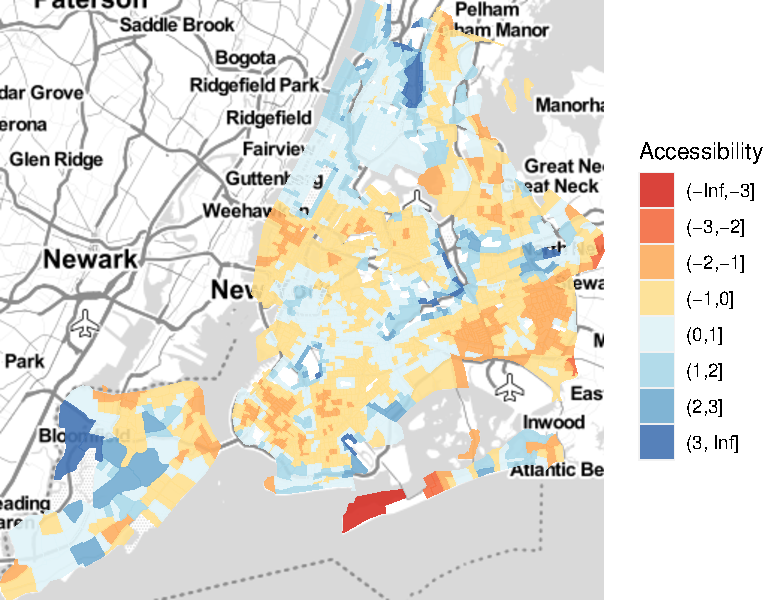
\includegraphics{map-1} \caption{Normalized utility-based park accessibility values in New York City.}\label{fig:map}
\end{figure*}

\hypertarget{model}{%
\subsection{Model}\label{model}}

\label{subsec:model}

We predict either the physical activity or the obesity rate (\(y\)) in a
census tract as a linear function of the tract's sociodemographic
characteristics \(X\) and accessibility to parks \(A\),
\begin{equation}\label{eq:themodel}
 y = X\beta + \beta_{a}A + \varepsilon
\end{equation}

As the observations are related to each other spatially, it is likely
that this process involves spatial spillovers of one kind or another. A
complete treatment of spatial econometrics is not warranted here; the
reader is directed to \citet{LeSage2009} as well as \citet{LeSage2014}.
Suffice it to say that the presence of spatial data generating processes
can negatively affect econometric interpretation in a variety of ways.
Each of these processes rely on spatial autoregression, where elements
of some random variable \(x\) are spatially dependent on other elements,
\begin{equation}\label{eq:autoregression}
 x = \rho W x + \varepsilon
\end{equation} with the strength of dependence an estimated parameter
\(\rho\), the structure of spatial dependence governed by the asserted
matrix \(W\) (details of \(W\) follow below), and some random
uncorrelated residual \(\varepsilon\). A collection of models is
available to represent spatial autodependence in the model residuals,
the independent variables, and the dependent variable.

The specific spatial model applied is both an econometric choice --- as
improperly specified spatial models can lead to inconsistent estimates
of model parameters and standard errors --- as well as a philosophical
choice about the likely structure of spillovers in the problem at hand.
In case of physical activity and obesity rates, we believe that the
outcomes are locally dependent: That is, a particular individual decides
whether or not to participate in physical activity independently of
whether his or her neighbors participate in physical activity. This does
not mean that we think it impossible that the socioeconomic variables of
neighboring tracts do not play a role. Mathematically, we assert that
the autodependence relationship on the dependent variable
\(y = \rho W y + \ldots\) has \(\rho = 0\) in the current case.

With this relationship ruled out, it remains a possibility that the
model residuals are spatially dependent, \begin{equation}\label{eq:SEM}
 y = X\beta + \beta_a A + u; u = \lambda W u + \varepsilon
\end{equation} that the outcome is partially dependent on the
socioeconomic variables in \emph{neighboring} tracts,
\begin{equation}\label{eq:SLX}
 y = X\beta + \beta_a A + W X \gamma + \varepsilon
\end{equation} or a linear combination of both.
\begin{equation}\label{eq:SDEM}
 y = X\beta + \beta_a A + W X \gamma + u; u = \lambda W u + \varepsilon 
\end{equation} These models are referred as the spatial error model
(SEM), the spatial lag of \(X\) model (SLX), and the spatial Durbin
error model (SDEM). \citet{Pace2008} suggest that a Hausman-style test
of the estimates of \(\beta\) derived from the OLS (Equation
\ref{eq:themodel}) and SEM (Equation \ref{eq:SEM}) can identify whether
the estimates are consistent. If the \(\beta\) estimates are dissimilar,
both specifications are inappropriate as they contain untreated omitted
variables. Similarly, if the SLX and SDEM estimates are dissimilar it is
an indication of missing variables in that specification. On the other
hand if the estimates of both pairs of models are similar and the
residual correlation parameter \(\lambda\) is non-zero, the model
accounting for spatially dependent residuals will produce proper
estimates of the model standard errors.

Note that in the lag-\(X\) specifications (SLX and SDEM) we exclude the
accessiblity component \(A\), that is we do \emph{not} consider that the
accessibility in a neighboring zone will have an effect on physical
activity or obesity rates. In a practical sense, this is because the
accessibility term \(A\) is itself spatially determined.

\hypertarget{spatial-weights}{%
\subsubsection{Spatial Weights}\label{spatial-weights}}

The spatial weights matrix \(W\) is constructed of individual elements
where \(w_{ij} = 0\) if observations \(i\) and \(j\) are spatially
independent of each other, and \(w_{ij} > 0\) if \(i\) and \(j\) are
spatially related in some way. \citet{Dubin1998} presents details on
constructing \(W\), but in this study we assume that tracts sharing at
least one common border point are neighbors of each other\footnote{We
  also considered a distance-discounted weights matrix, which produced
  similar results. This matrix is selected for simplicity.}. The
elements of \(W\) are then row-standardized so that each observation has
an equal total influence from all its neighbors.

\hypertarget{results}{%
\subsection{Results}\label{results}}

To determine which spatial effects specification was appropriate, we
estimated SLX and SDEM models of physical activity participation rates
as a function of tract covariates and accessibility. These two models
are presented in Table \ref{tab:slx-sdem}. With only a few exceptions,
the SLX and SDEM coefficient estimates for corresponding covariates lie
within the 95\% confidence intervals of the other model. A Hausman-style
test \citep{Pace2008} on the coefficients assumes a null hypothesis that
the coefficients are equivalent; this test produces \(p\)-value of only
\(0.03057\). Though this statistic is technically beneath a common
hypothesis test threshold of \(\alpha = 0.05\), we fail to reject the
null hypothesis that the coefficients are equivalent, as the differences
are at no point practically different from each other. The consequences
of rejecting the null hypothesis in this case would be to suggest a
model with spatial dependence of the dependent variable; as stated
above, we feel that such a relationship is unreasonable. As a
consequence of these analyses, we adopt the SDEM specification moving
forward as the spatial lag of the errors is significant and the overal
log likelihood of the SDEM is higher than the SLX specification.

\begin{table*}
\caption{Comparison of SLX and SDEM Coefficients}
\label{tab:slx-sdem}

\begin{tabular}{l c c}
\toprule
 & SLX & SDEM \\
\midrule
(Intercept)                         & $-35.3520 \; [-47.4781; -23.2260]^{*}$ & $-27.2048 \; [-45.0525; -9.3571]^{*}$ \\
log(Density)                        & $0.1057 \; [ -0.0920;   0.3034]$       & $0.2301 \; [  0.0646;  0.3956]^{*}$   \\
log(Income)                         & $6.4092 \; [  5.8339;   6.9845]^{*}$   & $6.2664 \; [  5.7721;  6.7607]^{*}$   \\
Fulltime                            & $0.1365 \; [  0.1130;   0.1601]^{*}$   & $0.1434 \; [  0.1221;  0.1647]^{*}$   \\
College-educated                    & $0.0371 \; [  0.0058;   0.0683]^{*}$   & $0.0313 \; [  0.0042;  0.0583]^{*}$   \\
Single Adults                       & $-0.0488 \; [ -0.0696;  -0.0279]^{*}$  & $-0.0472 \; [ -0.0659; -0.0284]^{*}$  \\
Youth (0-17)                        & $-0.1292 \; [ -0.1643;  -0.0941]^{*}$  & $-0.1300 \; [ -0.1608; -0.0992]^{*}$  \\
Young adults (18-34)                & $0.0395 \; [  0.0122;   0.0669]^{*}$   & $0.0387 \; [  0.0153;  0.0622]^{*}$   \\
Seniors (65+)                       & $0.0301 \; [ -0.0053;   0.0655]$       & $0.0354 \; [  0.0038;  0.0671]^{*}$   \\
Black population share              & $-0.0522 \; [ -0.0653;  -0.0391]^{*}$  & $-0.0536 \; [ -0.0641; -0.0432]^{*}$  \\
Asian population share              & $-0.0941 \; [ -0.1101;  -0.0781]^{*}$  & $-0.0954 \; [ -0.1081; -0.0827]^{*}$  \\
Hispanic population share           & $-0.1134 \; [ -0.1270;  -0.0998]^{*}$  & $-0.1152 \; [ -0.1261; -0.1044]^{*}$  \\
Other Minorities                    & $0.0154 \; [ -0.0957;   0.1265]$       & $-0.0119 \; [ -0.1145;  0.0906]$      \\
$\gamma$: log(Density)              & $1.6773 \; [  1.3277;   2.0269]^{*}$   & $1.1617 \; [  0.7470;  1.5764]^{*}$   \\
$\gamma$: log(Income)               & $1.9854 \; [  1.0562;   2.9146]^{*}$   & $1.6505 \; [  0.5414;  2.7597]^{*}$   \\
$\gamma$: Fulltime                  & $-0.0309 \; [ -0.0756;   0.0138]$      & $-0.0006 \; [ -0.0530;  0.0517]$      \\
$\gamma$: College-educated          & $-0.0002 \; [ -0.0545;   0.0541]$      & $-0.0174 \; [ -0.0819;  0.0471]$      \\
$\gamma$: Single Adults             & $-0.0390 \; [ -0.0764;  -0.0016]^{*}$  & $-0.0210 \; [ -0.0667;  0.0247]$      \\
$\gamma$: Youth (0-17)              & $0.0297 \; [ -0.0348;   0.0941]$       & $0.0205 \; [ -0.0552;  0.0962]$       \\
$\gamma$: Young adults (18-34)      & $0.1318 \; [  0.0847;   0.1789]^{*}$   & $0.0872 \; [  0.0319;  0.1424]^{*}$   \\
$\gamma$: Seniors (65+)             & $0.1505 \; [  0.0860;   0.2151]^{*}$   & $0.1181 \; [  0.0420;  0.1941]^{*}$   \\
$\gamma$: Black population share    & $0.0156 \; [ -0.0010;   0.0321]$       & $0.0102 \; [ -0.0073;  0.0278]$       \\
$\gamma$: Asian population share    & $-0.0325 \; [ -0.0521;  -0.0129]^{*}$  & $-0.0399 \; [ -0.0601; -0.0197]^{*}$  \\
$\gamma$: Hispanic population share & $-0.0028 \; [ -0.0201;   0.0144]$      & $0.0003 \; [ -0.0182;  0.0187]$       \\
$\gamma$: Other Minorities          & $0.2827 \; [  0.0215;   0.5438]^{*}$   & $0.1799 \; [ -0.1104;  0.4703]$       \\
Accessibility                       & $0.4522 \; [  0.3218;   0.5825]^{*}$   & $0.2076 \; [  0.0554;  0.3597]^{*}$   \\
$\lambda$: spatial correlation      &                                        & $0.5813 \; [  0.5344;  0.6282]^{*}$   \\
\midrule
Log Likelihood                      & $-5032.2042$                           & $-4786.9274$                          \\
Num. Obs.                           & $2099$                                 & $2099$                                \\
LR test: statistic                  & $$                                     & $490.5536$                            \\
LR test: p-value                    & $$                                     & $0.0000$                              \\
\bottomrule
\multicolumn{3}{l}{\scriptsize{$^*$ 0 outside the confidence interval. $y = $ tract-level physical activity rate.}}
\end{tabular}
\end{table*}

The coefficients in the SDEM model are of two general types: the direct
effect resulting from a tract's own attributes and the indirect effect
(\(\gamma\)) resulting from the spatially-weighted attributes of its
neighbors. For example, a percentage point increase in the share of
young adults in a tract increases the expected physical activity rate in
a tract by 0.03872 percentage points, and a percentage point increase in
the share of young adults \emph{in neighboring tracts} increases the
expected physical activity rate by an \emph{additional} 0.08718
percentage points. This opportunity to examine spatial spillovers of
attributes is a key benefit of using a spatial model.

For the most part the direct coefficients are highly significant and of
the expected sign. Tracts with higher shares of full-time workers,
college-educated adults, young adults, and high-income households all
show a greater share of individuals engaging in regular physical
activity. Conversely, tracts with greater population density and a
greater share of single adults, children, seniors, minorities, and low
income households all have lower modeled expected rates of physical
activity. The indirect coefficients are less clearly significant, with
only density, median tract income, some age groups, and some minority
groups showing an indirect effect.

Table \ref{tab:pa-models} presents the estimated spatial lag and
accessibility coefficients for three models using different
specifications of the utility equation, as well as the ten-minute walk
buffer calculated by ParkScore. Note that the model called ``Size and
Distance'' is precisely the model labeled ``SDEM'' in Table
\ref{tab:slx-sdem}. The controlling covariates are suppressed for
clarity but do not change meaningfully across the four specifications.
Complete model estimates are available in the Appendix. Each of the
three utility-based specifications is significant at the
\(\alpha = 0.05\) level or lower, and is of the hypothesized
directionality. That is, residents living in tracts with increased
utility-based accessiblity to green spaces show a significantly higher
physical activity participation rate. Taking the rough mean of the three
estimated utility-based coefficients, moving from the least-accessible
tract (\(A_i = -3\)) to the most-accessible tract (\(A_i = 3\)) is
expected to raise the physical activity rate by 1.2 percentage points.
With the understanding of the full 95\% confidence interval, we could
suggest that the true effect of excellent versus poor park access is
anywhere between 0.3 and 2.1 percentage points.

The 10-minute walk buffer is considerably less useful at isolating the
effects of park ``access'' on physical activity rates. As so few tracts
are located outside of the buffer, the standard error of the estimated
effect is large and implies an effect on activity rates anywhere from a
loss of 2.22 percentage points to a gain of 9.

\begin{table*}
\caption{Estimated Effect of Accessibility on Physical Activity Rates}
\label{tab:pa-models}

\begin{tabular}{l c c c c}
\toprule
 & Size and Distance & Twitter & Amenities & 10-Minute Walk \\
\midrule
Size and Distance & $0.2076^{*}$        &                     &                     &                      \\
                  & $ [0.0554; 0.3597]$ &                     &                     &                      \\
Amenities         &                     &                     & $0.1975^{*}$        &                      \\
                  &                     &                     & $ [0.0428; 0.3522]$ &                      \\
Twitter Activity  &                     & $0.2229^{*}$        &                     &                      \\
                  &                     & $ [0.0659; 0.3799]$ &                     &                      \\
10-minute walk    &                     &                     &                     & $0.5682$             \\
                  &                     &                     &                     & $ [-0.3638; 1.5001]$ \\
\midrule
Num. obs.         & $2099$              & $2099$              & $2099$              & $2099$               \\
Parameters        & $28$                & $28$                & $28$                & $28$                 \\
Log Likelihood    & $-4786.9274$        & $-4786.6411$        & $-4787.3677$        & $-4789.6660$         \\
\bottomrule
\multicolumn{5}{l}{\scriptsize{$^*$ 0 outside the confidence interval. 95\% confidence interval in brackets.}}
\end{tabular}
\end{table*}

We now consider the impacts of a model where the dependent variable is
the \emph{obesity} rate in a tract, and physical activity becomes an
independent covariate alongside the controlling variables and the
accessibility metrics. Table \ref{tab:obesity-models} presents estimates
of the effect of all three utility-based accessibility measures as well
as the 10-minute walk buffer. As before, the estimates of the other
variables are available in the Appendix. The correlation between
physical activity rates and obesity is clear; for every percentage point
increase in physical activity rate, the expected obesity rate drops by
\(0.43\) percentage points in all four accessiblity specifications. The
indirect effect of physical activity rates on obesity in neighboring
zones is inconsequential, supporting our methodological assertion that
public health variables are not spatially dependent, though the factors
leading to them may be.

As far as the accessibility values are concerned, none of the three
utility-based specifications nor the ParkScore 10-minute walk buffer are
correlated with obesity rates at the traditional 95\% confidence
interval. It is important to consider the implications of the full range
of the confidence interval, however \citep{Amrhein2019}. The results
suggest that after controlling for tract socioeconomic variables,
physical activity rates, and spatially correlated error terms, obesity
rates in tracts with excellent park accessibility are expected to be
between 0.9 percentage points lower and 0.0318 percentage points higher
than tracts with poor park accessibility. This range of values suggests
that accessibility to parks may have obesity-reducing effects beyond the
effect of accessibility on physical activity rates worth further study.

\begin{table*}
\caption{Estimated Effect of Accessibility on Obesity Rates}
\label{tab:obesity-models}

\begin{tabular}{l c c c c}
\toprule
 & Size and Distance & Twitter & Amenities & 10-Minute Walk \\
\midrule
Physical Activity           & $-0.4251^{*}$         & $-0.4250^{*}$         & $-0.4251^{*}$         & $-0.4256^{*}$         \\
                            & $ [-0.4463; -0.4039]$ & $ [-0.4462; -0.4038]$ & $ [-0.4463; -0.4039]$ & $ [-0.4468; -0.4045]$ \\
$\gamma$: Physical Activity & $-0.0321$             & $-0.0317$             & $-0.0318$             & $-0.0362$             \\
                            & $ [-0.0841;  0.0199]$ & $ [-0.0838;  0.0203]$ & $ [-0.0839;  0.0203]$ & $ [-0.0882;  0.0158]$ \\
Size and Distance           & $-0.0688$             &                       &                       &                       \\
                            & $ [-0.1440;  0.0064]$ &                       &                       &                       \\
Amenities                   &                       &                       & $-0.0695$             &                       \\
                            &                       &                       & $ [-0.1472;  0.0083]$ &                       \\
Twitter Activity            &                       & $-0.0731$             &                       &                       \\
                            &                       & $ [-0.1516;  0.0053]$ &                       &                       \\
10-minute walk              &                       &                       &                       & $-0.3573$             \\
                            &                       &                       &                       & $ [-0.7650;  0.0505]$ \\
\midrule
Num. obs.                   & $2099$                & $2099$                & $2099$                & $2099$                \\
Parameters                  & $30$                  & $30$                  & $30$                  & $30$                  \\
Log Likelihood              & $-3194.8851$          & $-3194.8268$          & $-3194.9556$          & $-3195.0152$          \\
\bottomrule
\multicolumn{5}{l}{\scriptsize{$^*$ 0 outside the confidence interval. 95\% confidence interval in brackets.}}
\end{tabular}
\end{table*}

\hypertarget{limitations-and-future-research-direction}{%
\section{Limitations and Future Research
Direction}\label{limitations-and-future-research-direction}}

We readily acknowledge limitations in this study. As in any study
conducted with areal data, we are at risk of falling victim to the
ecological inference fallacy, where aggregate statistics mask or
contradict disaggregated or individual-level trends. A large-sample
survey of individuals in New York City, including measured physical
activities and obesity would always be preferable to the tract-level
data used in this study. An ideal survey to address the question would
incorporate both sets of questions: physical activity and health data on
one hand and park use (including which parks were used and how
frequently) on the other. As no such dataset exists to our knowledge,
this tract-level aggregate analysis with asserted and transferred
utility coefficients is the possibility that remains.

This paper applies a previously-presented but little-used accessibility
statistic that could, in theory, accommodate many attributes of the
destination parks as well as the people who might use them. As an
illustration: the park-going population could be separated into at least
four delineated clusters, each preferring different amenities of a park:

\begin{itemize}
 \item{runners and cyclists: long, interesting trail systems}
 \item{sports players: soccer fields, basketball courts, or baseball diamonds}
 \item{families with small children: water features and playgrounds}
 \item{casual users: water features, gardens, performances, etc.}
\end{itemize}

An analyst could then compute the utility-based accessibility for each
cluster with different utility values for each park's amenities, and
obtain a measure of a neighborhood's accessibility to park features that
its residents most care about. In this paper, we proceed only
incrementally towards this by adding Twitter activity and some selected
park amenities as an element of each park's attractiveness above and
beyond its size. Exploring detailed definitions of an increased number
of amenities on one hand, and market segmentation strategies on the
other, could provide a more nuanced understanding of the relationship
between park accessibility and health outcomes.

As a travel impedance measure, we used the Euclidean distance between
each tract's population-weighted centroid and the nearest point on the
edge of a park's border. Euclidean distances have well-rehearsed
limitations regarding their fidelity with the underlying infrastructure
network, etc. Network-based distances can also suffer from challenges
when applied to multimodal problems; these challenges are exacerbated
when the non-highway mode share is high, as is likely when considering
access to parks. A better metric of travel impedance may be a mode
choice model logsum, which weights all alternative travel alternatives
against each other. We leave this as a recommendation for future
research.

We compared our utility-based accessibility to a well-constructed
isochrone that has attracted attention in the literature. That said,
virtually all tracts in New York City are within this specific
isochrone. It is possible that this isochrone may be more discriminating
of park access in other cities, or that a different definition would
yield different results in New York City. This observation however
reinforces our suggestion that a measure explicitly based in the utility
of access is warranted.

Finally, this study is primarily focused on the hypothesis that
accessibility to parks encourages physical activity, which in turn
reduces obesity. There are a multitude of other hypotheses that might be
proposed and tested with the basic methodology we have employed here, or
competing explanations for the outcomes we have observed. It is
distinctly possible, for instance, that individuals who wish to exercise
regularly in parks choose to live near them. Given that the CDC models
informing the small-area obesity and physical activity estimates
presumably include variables likely to influence such preferences
(income, etc.), our investigation cannot isolate the preferences from
the effect. Controlling for such a self-selection effect would be
necessary to isolate the exogenous impacts of park access on obesity or
other health outcomes. And regarding these other variables: this study
did not consider potential relationships between park access and
hospitalization rates, life expectancy, respiratory disease, mental
health, or any number of potential beneficial outcomes hypothesized or
explored in the existing literature. Exploring these connections and
their underlying mechanisms should be a priority as city planners and
urban architects attempt to improve the quality of life of urban
residents in the future.

\hypertarget{conclusion}{%
\section{Conclusion}\label{conclusion}}

Increased physical activity and decreased obesity rates are critical
measures of improvement in public health. Although many have theorized
the link between park accessibility and these metrics, previous
literature has produced mixed findings, perhaps owing to the range of
variables modeled and the coarse spatial scale of the analyses. Using
New York City as a case study, we presented a holistic and flexible
measurement for park accessibility that compares the continuous distance
to all parks in the region, weighted against the size of the park and
its other amenities, with weights determinable through revealed
preferences. In terms of physical activity, we found a positive
relationship where the least park-accessible tracts have an expected
physical activity participation rate between 0.3 and 2.1 percentage
points lower than the most accessible tracts. We also found a suggestive
though not sigificant relationship between park accessiblity and
expected obesity rates \emph{in addition to} the effect of physical
activity participation.

In both cases a common, isochrone-based analysis estimated a
statistically weak relationship with greater uncertainty. Isochrone
analyses are relatively common in the literature, perhaps because of the
widespread availability of and training in GIS software. In spite of
their widespread use, isochrones are relatively limited in terms of both
their theoretical underpinnings and their flexibility to accommodate
attributes of parks beyond their proximity. And even proximity may not
be adequately handled, as the isochrone threshold may be arbitrarily
asserted by the researcher. The model we apply in this paper extends a
more comprehensive and flexible approach for measuring the impact of
park access on health outcomes. Adopting utility-based accessibilities
of the kind used in this study will allow researchers to encompass the
full range of park amenities in their accessibility analyses, and to
separate the definition of access from the study of its effects. This
will in turn enable planners to consider how multiple attributes of a
park --- from its location to its size to its amenities and beyond ---
benefit the health of the community the park serves.


\bibliographystyle{sageh.bst}
\bibliography{manuscript.bbl}

\appendix
\section{Appendix}

In this appendix we present the complete estimation results for the models 
relating different definitions of access to physical activity (in Table
\ref{tab:pa-fullmodels}) and to obesity (in Table \ref{tab:ob-fullmodels}). In
each case we also present a base model with no accessibility statistics for
comparison.







\begin{table*}
\caption{Estimated Effects of Accessibility and Controls on Physical Activity Rates}
\begin{center}
\scalebox{0.7}{
\begin{tabular}{l c c c c c}
\toprule
 & No Access & Size and Distance & Tweets & Attributes & 10-min walk \\
\midrule
(Intercept)                         & $-25.9256^{*}$         & $-27.2048^{*}$         & $-26.5608^{*}$         & $-27.2431^{*}$         & $-26.1786^{*}$         \\
                                    & $ [-43.9792; -7.8720]$ & $ [-45.0525; -9.3571]$ & $ [-44.3812; -8.7404]$ & $ [-45.1016; -9.3846]$ & $ [-44.2194; -8.1378]$ \\
log(Density)                        & $0.2249^{*}$           & $0.2301^{*}$           & $0.2280^{*}$           & $0.2281^{*}$           & $0.2201^{*}$           \\
                                    & $ [  0.0594;  0.3905]$ & $ [  0.0646;  0.3956]$ & $ [  0.0626;  0.3934]$ & $ [  0.0626;  0.3936]$ & $ [  0.0544;  0.3858]$ \\
log(Income)                         & $6.2290^{*}$           & $6.2664^{*}$           & $6.2575^{*}$           & $6.2632^{*}$           & $6.2277^{*}$           \\
                                    & $ [  5.7342;  6.7239]$ & $ [  5.7721;  6.7607]$ & $ [  5.7636;  6.7513]$ & $ [  5.7688;  6.7575]$ & $ [  5.7331;  6.7224]$ \\
Fulltime                            & $0.1442^{*}$           & $0.1434^{*}$           & $0.1434^{*}$           & $0.1433^{*}$           & $0.1444^{*}$           \\
                                    & $ [  0.1228;  0.1656]$ & $ [  0.1221;  0.1647]$ & $ [  0.1220;  0.1647]$ & $ [  0.1220;  0.1646]$ & $ [  0.1230;  0.1658]$ \\
College-educated                    & $0.0307^{*}$           & $0.0313^{*}$           & $0.0316^{*}$           & $0.0307^{*}$           & $0.0315^{*}$           \\
                                    & $ [  0.0036;  0.0578]$ & $ [  0.0042;  0.0583]$ & $ [  0.0046;  0.0586]$ & $ [  0.0036;  0.0577]$ & $ [  0.0043;  0.0586]$ \\
Single Adults                       & $-0.0475^{*}$          & $-0.0472^{*}$          & $-0.0474^{*}$          & $-0.0469^{*}$          & $-0.0478^{*}$          \\
                                    & $ [ -0.0663; -0.0287]$ & $ [ -0.0659; -0.0284]$ & $ [ -0.0661; -0.0286]$ & $ [ -0.0657; -0.0282]$ & $ [ -0.0667; -0.0290]$ \\
Youth (0-17)                        & $-0.1302^{*}$          & $-0.1300^{*}$          & $-0.1304^{*}$          & $-0.1300^{*}$          & $-0.1307^{*}$          \\
                                    & $ [ -0.1611; -0.0993]$ & $ [ -0.1608; -0.0992]$ & $ [ -0.1611; -0.0996]$ & $ [ -0.1608; -0.0992]$ & $ [ -0.1615; -0.0998]$ \\
Young adults (18-34)                & $0.0372^{*}$           & $0.0387^{*}$           & $0.0387^{*}$           & $0.0388^{*}$           & $0.0370^{*}$           \\
                                    & $ [  0.0137;  0.0606]$ & $ [  0.0153;  0.0622]$ & $ [  0.0153;  0.0621]$ & $ [  0.0153;  0.0622]$ & $ [  0.0135;  0.0605]$ \\
Seniors (65+)                       & $0.0384^{*}$           & $0.0354^{*}$           & $0.0348^{*}$           & $0.0359^{*}$           & $0.0380^{*}$           \\
                                    & $ [  0.0068;  0.0701]$ & $ [  0.0038;  0.0671]$ & $ [  0.0032;  0.0664]$ & $ [  0.0043;  0.0675]$ & $ [  0.0064;  0.0697]$ \\
Black population share              & $-0.0537^{*}$          & $-0.0536^{*}$          & $-0.0536^{*}$          & $-0.0535^{*}$          & $-0.0535^{*}$          \\
                                    & $ [ -0.0642; -0.0433]$ & $ [ -0.0641; -0.0432]$ & $ [ -0.0640; -0.0432]$ & $ [ -0.0639; -0.0431]$ & $ [ -0.0639; -0.0430]$ \\
Asian population share              & $-0.0961^{*}$          & $-0.0954^{*}$          & $-0.0954^{*}$          & $-0.0955^{*}$          & $-0.0963^{*}$          \\
                                    & $ [ -0.1088; -0.0834]$ & $ [ -0.1081; -0.0827]$ & $ [ -0.1081; -0.0827]$ & $ [ -0.1082; -0.0829]$ & $ [ -0.1090; -0.0837]$ \\
Hispanic population share           & $-0.1148^{*}$          & $-0.1152^{*}$          & $-0.1153^{*}$          & $-0.1153^{*}$          & $-0.1147^{*}$          \\
                                    & $ [ -0.1256; -0.1039]$ & $ [ -0.1261; -0.1044]$ & $ [ -0.1261; -0.1044]$ & $ [ -0.1261; -0.1044]$ & $ [ -0.1255; -0.1038]$ \\
Other Minorities                    & $-0.0161$              & $-0.0119$              & $-0.0126$              & $-0.0115$              & $-0.0170$              \\
                                    & $ [ -0.1190;  0.0867]$ & $ [ -0.1145;  0.0906]$ & $ [ -0.1151;  0.0899]$ & $ [ -0.1141;  0.0910]$ & $ [ -0.1199;  0.0858]$ \\
$\gamma$: log(Density)              & $1.1804^{*}$           & $1.1617^{*}$           & $1.1491^{*}$           & $1.1685^{*}$           & $1.1668^{*}$           \\
                                    & $ [  0.7624;  1.5984]$ & $ [  0.7470;  1.5764]$ & $ [  0.7341;  1.5642]$ & $ [  0.7539;  1.5831]$ & $ [  0.7484;  1.5851]$ \\
$\gamma$: log(Income)               & $1.5660^{*}$           & $1.6505^{*}$           & $1.6211^{*}$           & $1.6398^{*}$           & $1.5611^{*}$           \\
                                    & $ [  0.4473;  2.6848]$ & $ [  0.5414;  2.7597]$ & $ [  0.5135;  2.7288]$ & $ [  0.5305;  2.7491]$ & $ [  0.4433;  2.6790]$ \\
$\gamma$: Fulltime                  & $0.0029$               & $-0.0006$              & $-0.0009$              & $0.0002$               & $0.0025$               \\
                                    & $ [ -0.0498;  0.0556]$ & $ [ -0.0530;  0.0517]$ & $ [ -0.0532;  0.0514]$ & $ [ -0.0521;  0.0525]$ & $ [ -0.0502;  0.0551]$ \\
$\gamma$: College-educated          & $-0.0190$              & $-0.0174$              & $-0.0163$              & $-0.0193$              & $-0.0212$              \\
                                    & $ [ -0.0842;  0.0461]$ & $ [ -0.0819;  0.0471]$ & $ [ -0.0808;  0.0482]$ & $ [ -0.0839;  0.0452]$ & $ [ -0.0863;  0.0440]$ \\
$\gamma$: Single Adults             & $-0.0218$              & $-0.0210$              & $-0.0218$              & $-0.0198$              & $-0.0215$              \\
                                    & $ [ -0.0680;  0.0243]$ & $ [ -0.0667;  0.0247]$ & $ [ -0.0674;  0.0239]$ & $ [ -0.0655;  0.0259]$ & $ [ -0.0676;  0.0246]$ \\
$\gamma$: Youth (0-17)              & $0.0169$               & $0.0205$               & $0.0200$               & $0.0217$               & $0.0161$               \\
                                    & $ [ -0.0594;  0.0932]$ & $ [ -0.0552;  0.0962]$ & $ [ -0.0557;  0.0956]$ & $ [ -0.0540;  0.0975]$ & $ [ -0.0602;  0.0923]$ \\
$\gamma$: Young adults (18-34)      & $0.0827^{*}$           & $0.0872^{*}$           & $0.0872^{*}$           & $0.0884^{*}$           & $0.0823^{*}$           \\
                                    & $ [  0.0270;  0.1384]$ & $ [  0.0319;  0.1424]$ & $ [  0.0320;  0.1425]$ & $ [  0.0331;  0.1437]$ & $ [  0.0267;  0.1380]$ \\
$\gamma$: Seniors (65+)             & $0.1207^{*}$           & $0.1181^{*}$           & $0.1161^{*}$           & $0.1198^{*}$           & $0.1204^{*}$           \\
                                    & $ [  0.0440;  0.1974]$ & $ [  0.0420;  0.1941]$ & $ [  0.0400;  0.1921]$ & $ [  0.0437;  0.1958]$ & $ [  0.0438;  0.1971]$ \\
$\gamma$: Black population share    & $0.0096$               & $0.0102$               & $0.0104$               & $0.0099$               & $0.0096$               \\
                                    & $ [ -0.0081;  0.0273]$ & $ [ -0.0073;  0.0278]$ & $ [ -0.0071;  0.0279]$ & $ [ -0.0077;  0.0274]$ & $ [ -0.0081;  0.0273]$ \\
$\gamma$: Asian population share    & $-0.0429^{*}$          & $-0.0399^{*}$          & $-0.0398^{*}$          & $-0.0405^{*}$          & $-0.0428^{*}$          \\
                                    & $ [ -0.0631; -0.0226]$ & $ [ -0.0601; -0.0197]$ & $ [ -0.0599; -0.0196]$ & $ [ -0.0606; -0.0203]$ & $ [ -0.0630; -0.0225]$ \\
$\gamma$: Hispanic population share & $0.0026$               & $0.0003$               & $0.0001$               & $0.0002$               & $0.0025$               \\
                                    & $ [ -0.0160;  0.0212]$ & $ [ -0.0182;  0.0187]$ & $ [ -0.0184;  0.0185]$ & $ [ -0.0183;  0.0186]$ & $ [ -0.0161;  0.0210]$ \\
$\gamma$: Other Minorities          & $0.1695$               & $0.1799$               & $0.1770$               & $0.1798$               & $0.1756$               \\
                                    & $ [ -0.1225;  0.4616]$ & $ [ -0.1104;  0.4703]$ & $ [ -0.1132;  0.4672]$ & $ [ -0.1106;  0.4702]$ & $ [ -0.1165;  0.4677]$ \\
$\lambda$: spatial correlation      & $0.5920^{*}$           & $0.5813^{*}$           & $0.5809^{*}$           & $0.5815^{*}$           & $0.5914^{*}$           \\
                                    & $ [  0.5458;  0.6382]$ & $ [  0.5344;  0.6282]$ & $ [  0.5339;  0.6278]$ & $ [  0.5346;  0.6284]$ & $ [  0.5451;  0.6376]$ \\
Size and Distance                   &                        & $0.2076^{*}$           &                        &                        &                        \\
                                    &                        & $ [  0.0554;  0.3597]$ &                        &                        &                        \\
Tweets                              &                        &                        & $0.2229^{*}$           &                        &                        \\
                                    &                        &                        & $ [  0.0659;  0.3799]$ &                        &                        \\
Attributes                          &                        &                        &                        & $0.1975^{*}$           &                        \\
                                    &                        &                        &                        & $ [  0.0428;  0.3522]$ &                        \\
10-min walk                         &                        &                        &                        &                        & $0.5682$               \\
                                    &                        &                        &                        &                        & $ [ -0.3638;  1.5001]$ \\
\midrule
Num. obs.                           & $2099$                 & $2099$                 & $2099$                 & $2099$                 & $2099$                 \\
Parameters                          & $27$                   & $28$                   & $28$                   & $28$                   & $28$                   \\
Log Likelihood                      & $-4790.3792$           & $-4786.9274$           & $-4786.6411$           & $-4787.3677$           & $-4789.6660$           \\
\bottomrule
\multicolumn{6}{l}{\scriptsize{$^*$ 0 outside the confidence interval. 95\% confidence interval in brackets.}}
\end{tabular}
}
\label{tab:pa-fullmodels}
\end{center}
\end{table*}




\begin{table*}
\caption{Estimated Effects of Accessibility and Controls on Obesity Rates}
\begin{center}
\scalebox{0.7}{
\begin{tabular}{l c c c c c}
\toprule
 & No Access & Size and Distance & Twitter & Amenities & 10-Minute Walk \\
\midrule
(Intercept)                         & $69.6657^{*}$         & $69.9773^{*}$         & $69.8388^{*}$         & $69.9833^{*}$         & $69.7516^{*}$         \\
                                    & $ [59.1228; 80.2086]$ & $ [59.4547; 80.4999]$ & $ [59.3196; 80.3579]$ & $ [59.4480; 80.5185]$ & $ [59.2183; 80.2850]$ \\
log(Density)                        & $-0.0343$             & $-0.0370$             & $-0.0366$             & $-0.0367$             & $-0.0305$             \\
                                    & $ [-0.1115;  0.0429]$ & $ [-0.1141;  0.0402]$ & $ [-0.1137;  0.0406]$ & $ [-0.1139;  0.0404]$ & $ [-0.1078;  0.0467]$ \\
log(Income)                         & $-0.3886^{*}$         & $-0.4015^{*}$         & $-0.4001^{*}$         & $-0.4021^{*}$         & $-0.3882^{*}$         \\
                                    & $ [-0.6649; -0.1122]$ & $ [-0.6780; -0.1251]$ & $ [-0.6765; -0.1238]$ & $ [-0.6786; -0.1256]$ & $ [-0.6643; -0.1121]$ \\
Fulltime                            & $-0.0117^{*}$         & $-0.0116^{*}$         & $-0.0116^{*}$         & $-0.0116^{*}$         & $-0.0119^{*}$         \\
                                    & $ [-0.0227; -0.0007]$ & $ [-0.0226; -0.0006]$ & $ [-0.0226; -0.0006]$ & $ [-0.0225; -0.0006]$ & $ [-0.0229; -0.0009]$ \\
College-educated                    & $0.0372^{*}$          & $0.0371^{*}$          & $0.0370^{*}$          & $0.0372^{*}$          & $0.0367^{*}$          \\
                                    & $ [ 0.0237;  0.0506]$ & $ [ 0.0236;  0.0505]$ & $ [ 0.0235;  0.0504]$ & $ [ 0.0237;  0.0506]$ & $ [ 0.0233;  0.0502]$ \\
Single Adults                       & $0.0017$              & $0.0017$              & $0.0018$              & $0.0017$              & $0.0019$              \\
                                    & $ [-0.0078;  0.0112]$ & $ [-0.0078;  0.0112]$ & $ [-0.0077;  0.0113]$ & $ [-0.0078;  0.0112]$ & $ [-0.0076;  0.0114]$ \\
Youth (0-17)                        & $0.0074$              & $0.0075$              & $0.0076$              & $0.0075$              & $0.0077$              \\
                                    & $ [-0.0080;  0.0227]$ & $ [-0.0078;  0.0228]$ & $ [-0.0077;  0.0230]$ & $ [-0.0078;  0.0229]$ & $ [-0.0076;  0.0231]$ \\
Young adults (18-34)                & $-0.0119^{*}$         & $-0.0125^{*}$         & $-0.0125^{*}$         & $-0.0125^{*}$         & $-0.0118^{*}$         \\
                                    & $ [-0.0234; -0.0005]$ & $ [-0.0239; -0.0010]$ & $ [-0.0239; -0.0010]$ & $ [-0.0240; -0.0011]$ & $ [-0.0232; -0.0004]$ \\
Seniors (65+)                       & $-0.0896^{*}$         & $-0.0886^{*}$         & $-0.0884^{*}$         & $-0.0887^{*}$         & $-0.0894^{*}$         \\
                                    & $ [-0.1052; -0.0740]$ & $ [-0.1042; -0.0730]$ & $ [-0.1040; -0.0728]$ & $ [-0.1043; -0.0731]$ & $ [-0.1050; -0.0738]$ \\
Black population share              & $0.0533^{*}$          & $0.0533^{*}$          & $0.0533^{*}$          & $0.0533^{*}$          & $0.0532^{*}$          \\
                                    & $ [ 0.0483;  0.0583]$ & $ [ 0.0484;  0.0583]$ & $ [ 0.0483;  0.0583]$ & $ [ 0.0483;  0.0582]$ & $ [ 0.0482;  0.0581]$ \\
Asian population share              & $-0.1043^{*}$         & $-0.1044^{*}$         & $-0.1044^{*}$         & $-0.1044^{*}$         & $-0.1042^{*}$         \\
                                    & $ [-0.1106; -0.0981]$ & $ [-0.1107; -0.0982]$ & $ [-0.1107; -0.0982]$ & $ [-0.1106; -0.0982]$ & $ [-0.1104; -0.0979]$ \\
Hispanic population share           & $-0.0042$             & $-0.0039$             & $-0.0039$             & $-0.0039$             & $-0.0042$             \\
                                    & $ [-0.0098;  0.0014]$ & $ [-0.0095;  0.0017]$ & $ [-0.0095;  0.0018]$ & $ [-0.0096;  0.0017]$ & $ [-0.0098;  0.0014]$ \\
Other Minorities                    & $-0.0639^{*}$         & $-0.0650^{*}$         & $-0.0650^{*}$         & $-0.0652^{*}$         & $-0.0632^{*}$         \\
                                    & $ [-0.1141; -0.0137]$ & $ [-0.1152; -0.0149]$ & $ [-0.1152; -0.0149]$ & $ [-0.1153; -0.0150]$ & $ [-0.1134; -0.0131]$ \\
Physical Activity Rate              & $-0.5805^{*}$         & $-0.5825^{*}$         & $-0.5808^{*}$         & $-0.5834^{*}$         & $-0.5674^{*}$         \\
                                    & $ [-0.8179; -0.3431]$ & $ [-0.8193; -0.3456]$ & $ [-0.8176; -0.3439]$ & $ [-0.8205; -0.3463]$ & $ [-0.8050; -0.3298]$ \\
$\gamma$: log(Density)              & $0.0755$              & $0.0372$              & $0.0407$              & $0.0388$              & $0.0880$              \\
                                    & $ [-0.6347;  0.7857]$ & $ [-0.6728;  0.7473]$ & $ [-0.6691;  0.7504]$ & $ [-0.6718;  0.7494]$ & $ [-0.6217;  0.7976]$ \\
$\gamma$: log(Income)               & $-0.0010$             & $-0.0005$             & $-0.0004$             & $-0.0007$             & $-0.0007$             \\
                                    & $ [-0.0302;  0.0282]$ & $ [-0.0296;  0.0287]$ & $ [-0.0295;  0.0288]$ & $ [-0.0299;  0.0284]$ & $ [-0.0299;  0.0285]$ \\
$\gamma$: Fulltime                  & $0.0869^{*}$          & $0.0867^{*}$          & $0.0864^{*}$          & $0.0870^{*}$          & $0.0885^{*}$          \\
                                    & $ [ 0.0505;  0.1233]$ & $ [ 0.0504;  0.1230]$ & $ [ 0.0501;  0.1228]$ & $ [ 0.0506;  0.1233]$ & $ [ 0.0521;  0.1250]$ \\
$\gamma$: College-educated          & $-0.0108$             & $-0.0107$             & $-0.0106$             & $-0.0109$             & $-0.0112$             \\
                                    & $ [-0.0365;  0.0150]$ & $ [-0.0364;  0.0149]$ & $ [-0.0363;  0.0151]$ & $ [-0.0367;  0.0148]$ & $ [-0.0369;  0.0146]$ \\
$\gamma$: Single Adults             & $-0.0356$             & $-0.0359$             & $-0.0356$             & $-0.0362$             & $-0.0351$             \\
                                    & $ [-0.0777;  0.0065]$ & $ [-0.0779;  0.0061]$ & $ [-0.0776;  0.0064]$ & $ [-0.0782;  0.0059]$ & $ [-0.0772;  0.0070]$ \\
$\gamma$: Youth (0-17)              & $-0.0296$             & $-0.0312^{*}$         & $-0.0312^{*}$         & $-0.0315^{*}$         & $-0.0291$             \\
                                    & $ [-0.0605;  0.0014]$ & $ [-0.0622; -0.0002]$ & $ [-0.0622; -0.0002]$ & $ [-0.0626; -0.0005]$ & $ [-0.0601;  0.0018]$ \\
$\gamma$: Young adults (18-34)      & $-0.0276$             & $-0.0266$             & $-0.0260$             & $-0.0270$             & $-0.0275$             \\
                                    & $ [-0.0690;  0.0138]$ & $ [-0.0680;  0.0147]$ & $ [-0.0674;  0.0154]$ & $ [-0.0684;  0.0144]$ & $ [-0.0689;  0.0139]$ \\
$\gamma$: Seniors (65+)             & $0.0155^{*}$          & $0.0154^{*}$          & $0.0154^{*}$          & $0.0155^{*}$          & $0.0153^{*}$          \\
                                    & $ [ 0.0050;  0.0259]$ & $ [ 0.0051;  0.0258]$ & $ [ 0.0050;  0.0258]$ & $ [ 0.0051;  0.0259]$ & $ [ 0.0049;  0.0258]$ \\
$\gamma$: Black population share    & $-0.0504^{*}$         & $-0.0509^{*}$         & $-0.0509^{*}$         & $-0.0507^{*}$         & $-0.0506^{*}$         \\
                                    & $ [-0.0640; -0.0368]$ & $ [-0.0645; -0.0373]$ & $ [-0.0645; -0.0373]$ & $ [-0.0643; -0.0371]$ & $ [-0.0642; -0.0371]$ \\
$\gamma$: Asian population share    & $0.0214^{*}$          & $0.0226^{*}$          & $0.0227^{*}$          & $0.0226^{*}$          & $0.0215^{*}$          \\
                                    & $ [ 0.0088;  0.0341]$ & $ [ 0.0099;  0.0353]$ & $ [ 0.0100;  0.0354]$ & $ [ 0.0099;  0.0354]$ & $ [ 0.0088;  0.0342]$ \\
$\gamma$: Hispanic population share & $0.0707$              & $0.0691$              & $0.0693$              & $0.0692$              & $0.0670$              \\
                                    & $ [-0.0777;  0.2190]$ & $ [-0.0791;  0.2173]$ & $ [-0.0789;  0.2175]$ & $ [-0.0790;  0.2174]$ & $ [-0.0813;  0.2153]$ \\
$\gamma$: Other Minorities          & $-0.4259^{*}$         & $-0.4251^{*}$         & $-0.4250^{*}$         & $-0.4251^{*}$         & $-0.4256^{*}$         \\
                                    & $ [-0.4471; -0.4047]$ & $ [-0.4463; -0.4039]$ & $ [-0.4462; -0.4038]$ & $ [-0.4463; -0.4039]$ & $ [-0.4468; -0.4045]$ \\
$\gamma$: Physical Activity Rate    & $-0.0351$             & $-0.0321$             & $-0.0317$             & $-0.0318$             & $-0.0362$             \\
                                    & $ [-0.0872;  0.0169]$ & $ [-0.0841;  0.0199]$ & $ [-0.0838;  0.0203]$ & $ [-0.0839;  0.0203]$ & $ [-0.0882;  0.0158]$ \\
$\lambda$: spatial correlation      & $0.8003^{*}$          & $0.7988^{*}$          & $0.7988^{*}$          & $0.7998^{*}$          & $0.8001^{*}$          \\
                                    & $ [ 0.7706;  0.8301]$ & $ [ 0.7689;  0.8287]$ & $ [ 0.7689;  0.8287]$ & $ [ 0.7700;  0.8296]$ & $ [ 0.7703;  0.8299]$ \\
Size and Distance                   &                       & $-0.0688$             &                       &                       &                       \\
                                    &                       & $ [-0.1440;  0.0064]$ &                       &                       &                       \\
Tweets                              &                       &                       & $-0.0731$             &                       &                       \\
                                    &                       &                       & $ [-0.1516;  0.0053]$ &                       &                       \\
Attributes                          &                       &                       &                       & $-0.0695$             &                       \\
                                    &                       &                       &                       & $ [-0.1472;  0.0083]$ &                       \\
10-min walk                         &                       &                       &                       &                       & $-0.3573$             \\
                                    &                       &                       &                       &                       & $ [-0.7650;  0.0505]$ \\
\midrule
Num. obs.                           & $2099$                & $2099$                & $2099$                & $2099$                & $2099$                \\
Parameters                          & $29$                  & $30$                  & $30$                  & $30$                  & $30$                  \\
Log Likelihood                      & $-3196.4885$          & $-3194.8851$          & $-3194.8268$          & $-3194.9556$          & $-3195.0152$          \\
\bottomrule
\multicolumn{6}{l}{\scriptsize{$^*$ 0 outside the confidence interval. 95\% confidence interval in brackets.}}
\end{tabular}
}
\label{tab:ob-fullmodels}
\end{center}
\end{table*}


\end{document}
